\documentclass[1p]{elsarticle_modified}
%\bibliographystyle{elsarticle-num}

%\usepackage[colorlinks]{hyperref}
%\usepackage{abbrmath_seonhwa} %\Abb, \Ascr, \Acal ,\Abf, \Afrak
\usepackage{amsfonts}
\usepackage{amssymb}
\usepackage{amsmath}
\usepackage{amsthm}
\usepackage{scalefnt}
\usepackage{amsbsy}
\usepackage{kotex}
\usepackage{caption}
\usepackage{subfig}
\usepackage{color}
\usepackage{graphicx}
\usepackage{xcolor} %% white, black, red, green, blue, cyan, magenta, yellow
\usepackage{float}
\usepackage{setspace}
\usepackage{hyperref}

\usepackage{tikz}
\usetikzlibrary{arrows}

\usepackage{multirow}
\usepackage{array} % fixed length table
\usepackage{hhline}

%%%%%%%%%%%%%%%%%%%%%
\makeatletter
\renewcommand*\env@matrix[1][\arraystretch]{%
	\edef\arraystretch{#1}%
	\hskip -\arraycolsep
	\let\@ifnextchar\new@ifnextchar
	\array{*\c@MaxMatrixCols c}}
\makeatother %https://tex.stackexchange.com/questions/14071/how-can-i-increase-the-line-spacing-in-a-matrix
%%%%%%%%%%%%%%%

\usepackage[normalem]{ulem}

\newcommand{\msout}[1]{\ifmmode\text{\sout{\ensuremath{#1}}}\else\sout{#1}\fi}
%SOURCE: \msout is \stkout macro in https://tex.stackexchange.com/questions/20609/strikeout-in-math-mode

\newcommand{\cancel}[1]{
	\ifmmode
	{\color{red}\msout{#1}}
	\else
	{\color{red}\sout{#1}}
	\fi
}

\newcommand{\add}[1]{
	{\color{blue}\uwave{#1}}
}

\newcommand{\replace}[2]{
	\ifmmode
	{\color{red}\msout{#1}}{\color{blue}\uwave{#2}}
	\else
	{\color{red}\sout{#1}}{\color{blue}\uwave{#2}}
	\fi
}

\newcommand{\Sol}{\mathcal{S}} %segment
\newcommand{\D}{D} %diagram
\newcommand{\A}{\mathcal{A}} %arc


%%%%%%%%%%%%%%%%%%%%%%%%%%%%%5 test

\def\sl{\operatorname{\textup{SL}}(2,\Cbb)}
\def\psl{\operatorname{\textup{PSL}}(2,\Cbb)}
\def\quan{\mkern 1mu \triangleright \mkern 1mu}

\theoremstyle{definition}
\newtheorem{thm}{Theorem}[section]
\newtheorem{prop}[thm]{Proposition}
\newtheorem{lem}[thm]{Lemma}
\newtheorem{ques}[thm]{Question}
\newtheorem{cor}[thm]{Corollary}
\newtheorem{defn}[thm]{Definition}
\newtheorem{exam}[thm]{Example}
\newtheorem{rmk}[thm]{Remark}
\newtheorem{alg}[thm]{Algorithm}

\newcommand{\I}{\sqrt{-1}}
\begin{document}

%\begin{frontmatter}
%
%\title{Boundary parabolic representations of knots up to 8 crossings}
%
%%% Group authors per affiliation:
%\author{Yunhi Cho} 
%\address{Department of Mathematics, University of Seoul, Seoul, Korea}
%\ead{yhcho@uos.ac.kr}
%
%
%\author{Seonhwa Kim} %\fnref{s_kim}}
%\address{Center for Geometry and Physics, Institute for Basic Science, Pohang, 37673, Korea}
%\ead{ryeona17@ibs.re.kr}
%
%\author{Hyuk Kim}
%\address{Department of Mathematical Sciences, Seoul National University, Seoul 08826, Korea}
%\ead{hyukkim@snu.ac.kr}
%
%\author{Seokbeom Yoon}
%\address{Department of Mathematical Sciences, Seoul National University, Seoul, 08826,  Korea}
%\ead{sbyoon15@snu.ac.kr}
%
%\begin{abstract}
%We find all boundary parabolic representation of knots up to 8 crossings.
%
%\end{abstract}
%\begin{keyword}
%    \MSC[2010] 57M25 
%\end{keyword}
%
%\end{frontmatter}

%\linenumbers
%\tableofcontents
%
\newcommand\colored[1]{\textcolor{white}{\rule[-0.35ex]{0.8em}{1.4ex}}\kern-0.8em\color{red} #1}%
%\newcommand\colored[1]{\textcolor{white}{ #1}\kern-2.17ex	\textcolor{white}{ #1}\kern-1.81ex	\textcolor{white}{ #1}\kern-2.15ex\color{red}#1	}

{\Large $\underline{12a_{0575}~(K12a_{0575})}$}

\setlength{\tabcolsep}{10pt}
\renewcommand{\arraystretch}{1.6}
\vspace{1cm}\begin{tabular}{m{100pt}>{\centering\arraybackslash}m{274pt}}
\multirow{5}{120pt}{
	\centering
	\includegraphics[width=112pt]{../../../GIT/diagram.site/Diagrams/png/1376_12a_0575.png}\\
\ \ \ A knot diagram\footnotemark}&
\allowdisplaybreaks
\textbf{Linearized knot diagam} \\
\cline{2-2}
 &
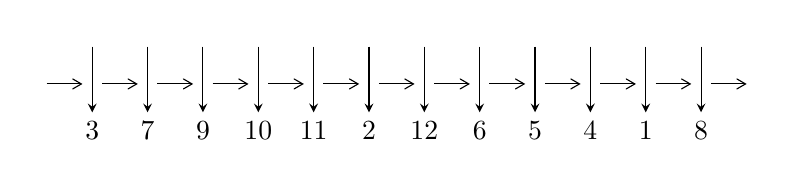
\begin{tikzpicture}[x=20pt, y=17pt]
	% nodes
	\node (C0) at (0, 0) {};
	\node (C1) at (1, 0) {};
	\node (C1U) at (1, +1) {};
	\node (C1D) at (1, -1) {3};

	\node (C2) at (2, 0) {};
	\node (C2U) at (2, +1) {};
	\node (C2D) at (2, -1) {7};

	\node (C3) at (3, 0) {};
	\node (C3U) at (3, +1) {};
	\node (C3D) at (3, -1) {9};

	\node (C4) at (4, 0) {};
	\node (C4U) at (4, +1) {};
	\node (C4D) at (4, -1) {10};

	\node (C5) at (5, 0) {};
	\node (C5U) at (5, +1) {};
	\node (C5D) at (5, -1) {11};

	\node (C6) at (6, 0) {};
	\node (C6U) at (6, +1) {};
	\node (C6D) at (6, -1) {2};

	\node (C7) at (7, 0) {};
	\node (C7U) at (7, +1) {};
	\node (C7D) at (7, -1) {12};

	\node (C8) at (8, 0) {};
	\node (C8U) at (8, +1) {};
	\node (C8D) at (8, -1) {6};

	\node (C9) at (9, 0) {};
	\node (C9U) at (9, +1) {};
	\node (C9D) at (9, -1) {5};

	\node (C10) at (10, 0) {};
	\node (C10U) at (10, +1) {};
	\node (C10D) at (10, -1) {4};

	\node (C11) at (11, 0) {};
	\node (C11U) at (11, +1) {};
	\node (C11D) at (11, -1) {1};

	\node (C12) at (12, 0) {};
	\node (C12U) at (12, +1) {};
	\node (C12D) at (12, -1) {8};
	\node (C13) at (13, 0) {};

	% arrows
	\draw[->,>={angle 60}]
	(C0) edge (C1) (C1) edge (C2) (C2) edge (C3) (C3) edge (C4) (C4) edge (C5) (C5) edge (C6) (C6) edge (C7) (C7) edge (C8) (C8) edge (C9) (C9) edge (C10) (C10) edge (C11) (C11) edge (C12) (C12) edge (C13) ;	\draw[->,>=stealth]
	(C1U) edge (C1D) (C2U) edge (C2D) (C3U) edge (C3D) (C4U) edge (C4D) (C5U) edge (C5D) (C6U) edge (C6D) (C7U) edge (C7D) (C8U) edge (C8D) (C9U) edge (C9D) (C10U) edge (C10D) (C11U) edge (C11D) (C12U) edge (C12D) ;
	\end{tikzpicture} \\
\hhline{~~} \\& 
\textbf{Solving Sequence} \\ \cline{2-2} 
 &
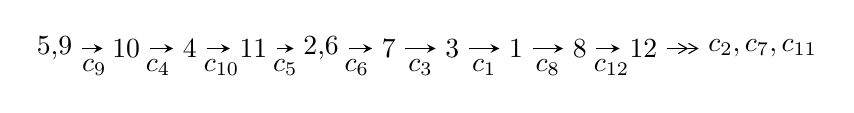
\begin{tikzpicture}[x=23pt, y=7pt]
	% node
	\node (A0) at (-1/8, 0) {5,9};
	\node (A1) at (1, 0) {10};
	\node (A2) at (2, 0) {4};
	\node (A3) at (3, 0) {11};
	\node (A4) at (65/16, 0) {2,6};
	\node (A5) at (41/8, 0) {7};
	\node (A6) at (49/8, 0) {3};
	\node (A7) at (57/8, 0) {1};
	\node (A8) at (65/8, 0) {8};
	\node (A9) at (73/8, 0) {12};
	\node (C1) at (1/2, -1) {$c_{9}$};
	\node (C2) at (3/2, -1) {$c_{4}$};
	\node (C3) at (5/2, -1) {$c_{10}$};
	\node (C4) at (7/2, -1) {$c_{5}$};
	\node (C5) at (37/8, -1) {$c_{6}$};
	\node (C6) at (45/8, -1) {$c_{3}$};
	\node (C7) at (53/8, -1) {$c_{1}$};
	\node (C8) at (61/8, -1) {$c_{8}$};
	\node (C9) at (69/8, -1) {$c_{12}$};
	\node (A10) at (11, 0) {$c_{2},c_{7},c_{11}$};

	% edge
	\draw[->,>=stealth]	
	(A0) edge (A1) (A1) edge (A2) (A2) edge (A3) (A3) edge (A4) (A4) edge (A5) (A5) edge (A6) (A6) edge (A7) (A7) edge (A8) (A8) edge (A9) ;
	\draw[->>,>={angle 60}]	
	(A9) edge (A10);
\end{tikzpicture} \\ 

\end{tabular} \\

\footnotetext{
The image of knot diagram is generated by the software ``\textbf{Draw programme}" developed by Andrew Bartholomew(\url{http://www.layer8.co.uk/maths/draw/index.htm\#Running-draw}), where we modified some parts for our purpose(\url{https://github.com/CATsTAILs/LinksPainter}).
}\phantom \\ \newline 
\centering \textbf{Ideals for irreducible components\footnotemark of $X_{\text{par}}$} 
 
\begin{align*}
I^u_{1}&=\langle 
-2 u^{37}+3 u^{36}+\cdots+b-3,\;-3 u^{39}+9 u^{38}+\cdots+2 a-10,\;u^{40}-3 u^{39}+\cdots+6 u-2\rangle \\
I^u_{2}&=\langle 
5150 u^{29} a-9644 u^{29}+\cdots-4195 a-8440,\;2 u^{29} a+u^{28}+\cdots+a+2,\;u^{30}+u^{29}+\cdots+u+1\rangle \\
I^u_{3}&=\langle 
b-1,\;-2 u^3+3 u^2+3 a-3 u+3,\;u^4+3 u^2+3\rangle \\
I^u_{4}&=\langle 
b+1,\;u^2+a- u+1,\;u^4+u^2-1\rangle \\
\\
I^v_{1}&=\langle 
a,\;b-1,\;v+1\rangle \\
\end{align*}
\raggedright * 5 irreducible components of $\dim_{\mathbb{C}}=0$, with total 109 representations.\\
\footnotetext{All coefficients of polynomials are rational numbers. But the coefficients are sometimes approximated in decimal forms when there is not enough margin.}
\newpage
\renewcommand{\arraystretch}{1}
\centering \section*{I. $I^u_{1}= \langle -2 u^{37}+3 u^{36}+\cdots+b-3,\;-3 u^{39}+9 u^{38}+\cdots+2 a-10,\;u^{40}-3 u^{39}+\cdots+6 u-2 \rangle$}
\flushleft \textbf{(i) Arc colorings}\\
\begin{tabular}{m{7pt} m{180pt} m{7pt} m{180pt} }
\flushright $a_{5}=$&$\begin{pmatrix}0\\u\end{pmatrix}$ \\
\flushright $a_{9}=$&$\begin{pmatrix}1\\0\end{pmatrix}$ \\
\flushright $a_{10}=$&$\begin{pmatrix}1\\u^2\end{pmatrix}$ \\
\flushright $a_{4}=$&$\begin{pmatrix}u\\u^3+u\end{pmatrix}$ \\
\flushright $a_{11}=$&$\begin{pmatrix}u^2+1\\u^4+2 u^2\end{pmatrix}$ \\
\flushright $a_{2}=$&$\begin{pmatrix}\frac{3}{2} u^{39}-\frac{9}{2} u^{38}+\cdots-\frac{17}{2} u+5\\2 u^{37}-3 u^{36}+\cdots-3 u+3\end{pmatrix}$ \\
\flushright $a_{6}=$&$\begin{pmatrix}- u^5-2 u^3- u\\- u^7-3 u^5-2 u^3+u\end{pmatrix}$ \\
\flushright $a_{7}=$&$\begin{pmatrix}-\frac{3}{2} u^{39}+\frac{5}{2} u^{38}+\cdots+\frac{5}{2} u-2\\- u^{39}+2 u^{38}+\cdots+3 u-1\end{pmatrix}$ \\
\flushright $a_{3}=$&$\begin{pmatrix}u^3+2 u\\u^3+u\end{pmatrix}$ \\
\flushright $a_{1}=$&$\begin{pmatrix}\frac{5}{2} u^{39}-\frac{15}{2} u^{38}+\cdots-\frac{33}{2} u+9\\3 u^{37}-5 u^{36}+\cdots-6 u+5\end{pmatrix}$ \\
\flushright $a_{8}=$&$\begin{pmatrix}- u^{12}-5 u^{10}-9 u^8-6 u^6+u^2+1\\- u^{14}-6 u^{12}-13 u^{10}-10 u^8+2 u^6+4 u^4- u^2\end{pmatrix}$ \\
\flushright $a_{12}=$&$\begin{pmatrix}-\frac{3}{2} u^{39}+\frac{9}{2} u^{38}+\cdots+\frac{21}{2} u-4\\-2 u^{37}+3 u^{36}+\cdots+4 u-3\end{pmatrix}$\\&\end{tabular}
\flushleft \textbf{(ii) Obstruction class $= -1$}\\~\\
\flushleft \textbf{(iii) Cusp Shapes $= 8 u^{39}-14 u^{38}+\cdots-20 u-8$}\\~\\
\newpage\renewcommand{\arraystretch}{1}
\flushleft \textbf{(iv) u-Polynomials at the component}\newline \\
\begin{tabular}{m{50pt}|m{274pt}}
Crossings & \hspace{64pt}u-Polynomials at each crossing \\
\hline $$\begin{aligned}c_{1},c_{11}\end{aligned}$$&$\begin{aligned}
&u^{40}+17 u^{39}+\cdots+19 u+1
\end{aligned}$\\
\hline $$\begin{aligned}c_{2},c_{6},c_{7}\\c_{12}\end{aligned}$$&$\begin{aligned}
&u^{40}- u^{39}+\cdots- u-1
\end{aligned}$\\
\hline $$\begin{aligned}c_{3},c_{5}\end{aligned}$$&$\begin{aligned}
&u^{40}-3 u^{39}+\cdots+10 u-2
\end{aligned}$\\
\hline $$\begin{aligned}c_{4},c_{9},c_{10}\end{aligned}$$&$\begin{aligned}
&u^{40}+3 u^{39}+\cdots-6 u-2
\end{aligned}$\\
\hline $$\begin{aligned}c_{8}\end{aligned}$$&$\begin{aligned}
&u^{40}-21 u^{39}+\cdots-6214 u+562
\end{aligned}$\\
\hline
\end{tabular}\\~\\
\newpage\renewcommand{\arraystretch}{1}
\flushleft \textbf{(v) Riley Polynomials at the component}\newline \\
\begin{tabular}{m{50pt}|m{274pt}}
Crossings & \hspace{64pt}Riley Polynomials at each crossing \\
\hline $$\begin{aligned}c_{1},c_{11}\end{aligned}$$&$\begin{aligned}
&y^{40}+23 y^{39}+\cdots-67 y+1
\end{aligned}$\\
\hline $$\begin{aligned}c_{2},c_{6},c_{7}\\c_{12}\end{aligned}$$&$\begin{aligned}
&y^{40}-17 y^{39}+\cdots-19 y+1
\end{aligned}$\\
\hline $$\begin{aligned}c_{3},c_{5}\end{aligned}$$&$\begin{aligned}
&y^{40}-27 y^{39}+\cdots+64 y+4
\end{aligned}$\\
\hline $$\begin{aligned}c_{4},c_{9},c_{10}\end{aligned}$$&$\begin{aligned}
&y^{40}+33 y^{39}+\cdots-32 y+4
\end{aligned}$\\
\hline $$\begin{aligned}c_{8}\end{aligned}$$&$\begin{aligned}
&y^{40}-3 y^{39}+\cdots-5405216 y+315844
\end{aligned}$\\
\hline
\end{tabular}\\~\\
\newpage\flushleft \textbf{(vi) Complex Volumes and Cusp Shapes}
$$\begin{array}{c|c|c}  
\text{Solutions to }I^u_{1}& \I (\text{vol} + \sqrt{-1}CS) & \text{Cusp shape}\\
 \hline 
\begin{aligned}
u &= \phantom{-}0.033946 + 1.113580 I \\
a &= -0.443213 + 0.659546 I \\
b &= -0.529000 - 0.069966 I\end{aligned}
 & \phantom{-}2.62973 - 1.45530 I & -8.41133 + 4.63856 I \\ \hline\begin{aligned}
u &= \phantom{-}0.033946 - 1.113580 I \\
a &= -0.443213 - 0.659546 I \\
b &= -0.529000 + 0.069966 I\end{aligned}
 & \phantom{-}2.62973 + 1.45530 I & -8.41133 - 4.63856 I \\ \hline\begin{aligned}
u &= \phantom{-}0.833882 + 0.049861 I \\
a &= \phantom{-}0.866824 + 0.530873 I \\
b &= \phantom{-}0.179877 + 0.772910 I\end{aligned}
 & -7.70738 + 2.92668 I & -18.8392 - 4.9556 I \\ \hline\begin{aligned}
u &= \phantom{-}0.833882 - 0.049861 I \\
a &= \phantom{-}0.866824 - 0.530873 I \\
b &= \phantom{-}0.179877 - 0.772910 I\end{aligned}
 & -7.70738 - 2.92668 I & -18.8392 + 4.9556 I \\ \hline\begin{aligned}
u &= \phantom{-}0.366756 + 1.108260 I \\
a &= \phantom{-}1.59722 + 0.00494 I \\
b &= \phantom{-}1.77944 + 1.15129 I\end{aligned}
 & -1.99390 + 8.37642 I & -14.1780 - 5.1626 I \\ \hline\begin{aligned}
u &= \phantom{-}0.366756 - 1.108260 I \\
a &= \phantom{-}1.59722 - 0.00494 I \\
b &= \phantom{-}1.77944 - 1.15129 I\end{aligned}
 & -1.99390 - 8.37642 I & -14.1780 + 5.1626 I \\ \hline\begin{aligned}
u &= \phantom{-}0.817179 + 0.133455 I \\
a &= -2.11445 + 2.81732 I \\
b &= -2.01736 + 1.18808 I\end{aligned}
 & -4.96679 - 12.67870 I & -17.0433 + 8.8234 I \\ \hline\begin{aligned}
u &= \phantom{-}0.817179 - 0.133455 I \\
a &= -2.11445 - 2.81732 I \\
b &= -2.01736 - 1.18808 I\end{aligned}
 & -4.96679 + 12.67870 I & -17.0433 - 8.8234 I \\ \hline\begin{aligned}
u &= \phantom{-}0.218298 + 1.152810 I \\
a &= -0.690017 + 0.431742 I \\
b &= -0.822252 - 0.487537 I\end{aligned}
 & \phantom{-}2.56813 - 1.57777 I & -7.38729 + 3.27205 I \\ \hline\begin{aligned}
u &= \phantom{-}0.218298 - 1.152810 I \\
a &= -0.690017 - 0.431742 I \\
b &= -0.822252 + 0.487537 I\end{aligned}
 & \phantom{-}2.56813 + 1.57777 I & -7.38729 - 3.27205 I\\
 \hline 
 \end{array}$$\newpage$$\begin{array}{c|c|c}  
\text{Solutions to }I^u_{1}& \I (\text{vol} + \sqrt{-1}CS) & \text{Cusp shape}\\
 \hline 
\begin{aligned}
u &= -0.813800\phantom{ +0.000000I} \\
a &= -1.17657\phantom{ +0.000000I} \\
b &= -0.516311\phantom{ +0.000000I}\end{aligned}
 & -5.88324\phantom{ +0.000000I} & -14.0450\phantom{ +0.000000I} \\ \hline\begin{aligned}
u &= \phantom{-}0.753305 + 0.134603 I \\
a &= \phantom{-}1.75806 - 1.14597 I \\
b &= \phantom{-}1.39356 - 0.37494 I\end{aligned}
 & -0.35694 - 2.08784 I & -11.36506 + 1.10964 I \\ \hline\begin{aligned}
u &= \phantom{-}0.753305 - 0.134603 I \\
a &= \phantom{-}1.75806 + 1.14597 I \\
b &= \phantom{-}1.39356 + 0.37494 I\end{aligned}
 & -0.35694 + 2.08784 I & -11.36506 - 1.10964 I \\ \hline\begin{aligned}
u &= \phantom{-}0.381450 + 1.215900 I \\
a &= -0.154097 + 0.151781 I \\
b &= -0.323421 + 0.861671 I\end{aligned}
 & -4.11653 - 7.29632 I & -12.0000 + 8.2173 I \\ \hline\begin{aligned}
u &= \phantom{-}0.381450 - 1.215900 I \\
a &= -0.154097 - 0.151781 I \\
b &= -0.323421 - 0.861671 I\end{aligned}
 & -4.11653 + 7.29632 I & -12.0000 - 8.2173 I \\ \hline\begin{aligned}
u &= -0.686189 + 0.170880 I \\
a &= \phantom{-}0.15715 + 2.12370 I \\
b &= \phantom{-}0.432447 + 0.716843 I\end{aligned}
 & \phantom{-}0.50362 + 4.50911 I & -12.14030 - 7.25109 I \\ \hline\begin{aligned}
u &= -0.686189 - 0.170880 I \\
a &= \phantom{-}0.15715 - 2.12370 I \\
b &= \phantom{-}0.432447 - 0.716843 I\end{aligned}
 & \phantom{-}0.50362 - 4.50911 I & -12.14030 + 7.25109 I \\ \hline\begin{aligned}
u &= -0.129451 + 0.688064 I \\
a &= -0.409921 + 0.548317 I \\
b &= -0.825583 + 0.231072 I\end{aligned}
 & \phantom{-}2.57797 - 1.26521 I & -7.12510 + 2.47533 I \\ \hline\begin{aligned}
u &= -0.129451 - 0.688064 I \\
a &= -0.409921 - 0.548317 I \\
b &= -0.825583 - 0.231072 I\end{aligned}
 & \phantom{-}2.57797 + 1.26521 I & -7.12510 - 2.47533 I \\ \hline\begin{aligned}
u &= -0.361326 + 1.266880 I \\
a &= \phantom{-}0.659360 + 0.462083 I \\
b &= \phantom{-}0.516491 - 0.026454 I\end{aligned}
 & -1.95240 + 4.22783 I & -12.00000 + 0. I\phantom{ +0.000000I}\\
 \hline 
 \end{array}$$\newpage$$\begin{array}{c|c|c}  
\text{Solutions to }I^u_{1}& \I (\text{vol} + \sqrt{-1}CS) & \text{Cusp shape}\\
 \hline 
\begin{aligned}
u &= -0.361326 - 1.266880 I \\
a &= \phantom{-}0.659360 - 0.462083 I \\
b &= \phantom{-}0.516491 + 0.026454 I\end{aligned}
 & -1.95240 - 4.22783 I & -12.00000 + 0. I\phantom{ +0.000000I} \\ \hline\begin{aligned}
u &= -0.391716 + 0.557095 I \\
a &= \phantom{-}0.438882 + 0.839532 I \\
b &= \phantom{-}1.51444 + 0.60899 I\end{aligned}
 & -0.63986 + 8.65751 I & -12.8507 - 9.2010 I \\ \hline\begin{aligned}
u &= -0.391716 - 0.557095 I \\
a &= \phantom{-}0.438882 - 0.839532 I \\
b &= \phantom{-}1.51444 - 0.60899 I\end{aligned}
 & -0.63986 - 8.65751 I & -12.8507 + 9.2010 I \\ \hline\begin{aligned}
u &= \phantom{-}0.373696 + 1.301330 I \\
a &= -0.998383 + 0.344441 I \\
b &= -0.072953 - 0.689963 I\end{aligned}
 & -3.49133 - 1.41285 I & \phantom{-0.000000 } 0 \\ \hline\begin{aligned}
u &= \phantom{-}0.373696 - 1.301330 I \\
a &= -0.998383 - 0.344441 I \\
b &= -0.072953 + 0.689963 I\end{aligned}
 & -3.49133 + 1.41285 I & \phantom{-0.000000 } 0 \\ \hline\begin{aligned}
u &= -0.212237 + 1.347650 I \\
a &= -0.30613 + 1.72945 I \\
b &= \phantom{-}1.070540 + 0.223660 I\end{aligned}
 & \phantom{-}3.73398 - 2.59581 I & \phantom{-0.000000 } 0 \\ \hline\begin{aligned}
u &= -0.212237 - 1.347650 I \\
a &= -0.30613 - 1.72945 I \\
b &= \phantom{-}1.070540 - 0.223660 I\end{aligned}
 & \phantom{-}3.73398 + 2.59581 I & \phantom{-0.000000 } 0 \\ \hline\begin{aligned}
u &= -0.542858 + 0.319373 I \\
a &= -1.52946 - 1.40938 I \\
b &= -1.067890 + 0.349863 I\end{aligned}
 & -1.40399 - 5.26208 I & -14.5220 + 2.7158 I \\ \hline\begin{aligned}
u &= -0.542858 - 0.319373 I \\
a &= -1.52946 + 1.40938 I \\
b &= -1.067890 - 0.349863 I\end{aligned}
 & -1.40399 + 5.26208 I & -14.5220 - 2.7158 I \\ \hline\begin{aligned}
u &= -0.289068 + 1.350620 I \\
a &= \phantom{-}0.94267 - 1.37582 I \\
b &= -0.525974 - 1.055320 I\end{aligned}
 & \phantom{-}5.28661 + 8.06862 I & \phantom{-0.000000 } 0\\
 \hline 
 \end{array}$$\newpage$$\begin{array}{c|c|c}  
\text{Solutions to }I^u_{1}& \I (\text{vol} + \sqrt{-1}CS) & \text{Cusp shape}\\
 \hline 
\begin{aligned}
u &= -0.289068 - 1.350620 I \\
a &= \phantom{-}0.94267 + 1.37582 I \\
b &= -0.525974 + 1.055320 I\end{aligned}
 & \phantom{-}5.28661 - 8.06862 I & \phantom{-0.000000 } 0 \\ \hline\begin{aligned}
u &= \phantom{-}0.322258 + 1.346450 I \\
a &= -0.02734 + 1.57117 I \\
b &= -1.65332 + 0.31762 I\end{aligned}
 & \phantom{-}4.30721 - 5.98911 I & \phantom{-0.000000 } 0 \\ \hline\begin{aligned}
u &= \phantom{-}0.322258 - 1.346450 I \\
a &= -0.02734 - 1.57117 I \\
b &= -1.65332 - 0.31762 I\end{aligned}
 & \phantom{-}4.30721 + 5.98911 I & \phantom{-0.000000 } 0 \\ \hline\begin{aligned}
u &= -0.018698 + 1.394080 I \\
a &= -0.777700 - 0.023034 I \\
b &= \phantom{-}1.34120 - 0.55017 I\end{aligned}
 & \phantom{-}8.78475 - 0.92619 I & \phantom{-0.000000 } 0 \\ \hline\begin{aligned}
u &= -0.018698 - 1.394080 I \\
a &= -0.777700 + 0.023034 I \\
b &= \phantom{-}1.34120 + 0.55017 I\end{aligned}
 & \phantom{-}8.78475 + 0.92619 I & \phantom{-0.000000 } 0 \\ \hline\begin{aligned}
u &= \phantom{-}0.353485 + 1.352330 I \\
a &= -0.60310 - 2.64696 I \\
b &= \phantom{-}2.18251 - 1.17429 I\end{aligned}
 & -0.2892 - 16.8986 I & \phantom{-0.000000 } 0 \\ \hline\begin{aligned}
u &= \phantom{-}0.353485 - 1.352330 I \\
a &= -0.60310 + 2.64696 I \\
b &= \phantom{-}2.18251 + 1.17429 I\end{aligned}
 & -0.2892 + 16.8986 I & \phantom{-0.000000 } 0 \\ \hline\begin{aligned}
u &= -0.075124 + 1.399150 I \\
a &= \phantom{-}1.270610 - 0.109417 I \\
b &= -1.96624 - 0.40727 I\end{aligned}
 & \phantom{-}5.50017 + 10.01410 I & \phantom{-0.000000 } 0 \\ \hline\begin{aligned}
u &= -0.075124 - 1.399150 I \\
a &= \phantom{-}1.270610 + 0.109417 I \\
b &= -1.96624 + 0.40727 I\end{aligned}
 & \phantom{-}5.50017 - 10.01410 I & \phantom{-0.000000 } 0 \\ \hline\begin{aligned}
u &= \phantom{-}0.318625\phantom{ +0.000000I} \\
a &= \phantom{-}0.902652\phantom{ +0.000000I} \\
b &= \phantom{-}0.303261\phantom{ +0.000000I}\end{aligned}
 & -0.549970\phantom{ +0.000000I} & -17.8990\phantom{ +0.000000I}\\
 \hline 
 \end{array}$$\newpage\newpage\renewcommand{\arraystretch}{1}
\centering \section*{II. $I^u_{2}= \langle 5150 u^{29} a-9644 u^{29}+\cdots-4195 a-8440,\;2 u^{29} a+u^{28}+\cdots+a+2,\;u^{30}+u^{29}+\cdots+u+1 \rangle$}
\flushleft \textbf{(i) Arc colorings}\\
\begin{tabular}{m{7pt} m{180pt} m{7pt} m{180pt} }
\flushright $a_{5}=$&$\begin{pmatrix}0\\u\end{pmatrix}$ \\
\flushright $a_{9}=$&$\begin{pmatrix}1\\0\end{pmatrix}$ \\
\flushright $a_{10}=$&$\begin{pmatrix}1\\u^2\end{pmatrix}$ \\
\flushright $a_{4}=$&$\begin{pmatrix}u\\u^3+u\end{pmatrix}$ \\
\flushright $a_{11}=$&$\begin{pmatrix}u^2+1\\u^4+2 u^2\end{pmatrix}$ \\
\flushright $a_{2}=$&$\begin{pmatrix}a\\-0.524066 a u^{29}+0.981378 u^{29}+\cdots+0.426885 a+0.858858\end{pmatrix}$ \\
\flushright $a_{6}=$&$\begin{pmatrix}- u^5-2 u^3- u\\- u^7-3 u^5-2 u^3+u\end{pmatrix}$ \\
\flushright $a_{7}=$&$\begin{pmatrix}-0.524066 a u^{29}+0.981378 u^{29}+\cdots-0.573115 a+0.858858\\-0.153658 a u^{29}-0.0850717 u^{29}+\cdots+0.387300 a+0.950850\end{pmatrix}$ \\
\flushright $a_{3}=$&$\begin{pmatrix}u^3+2 u\\u^3+u\end{pmatrix}$ \\
\flushright $a_{1}=$&$\begin{pmatrix}0.223873 a u^{29}+0.289508 u^{29}+\cdots+0.866185 a+0.429226\\-0.701537 a u^{29}+1.67915 u^{29}+\cdots+0.223873 a+1.28951\end{pmatrix}$ \\
\flushright $a_{8}=$&$\begin{pmatrix}- u^{12}-5 u^{10}-9 u^8-6 u^6+u^2+1\\- u^{14}-6 u^{12}-13 u^{10}-10 u^8+2 u^6+4 u^4- u^2\end{pmatrix}$ \\
\flushright $a_{12}=$&$\begin{pmatrix}-0.00142465 a u^{29}+0.311794 u^{29}+\cdots+0.896306 a+1.12272\\-0.0934161 a u^{29}+1.30192 u^{29}+\cdots-0.0850717 a+1.18999\end{pmatrix}$\\&\end{tabular}
\flushleft \textbf{(ii) Obstruction class $= -1$}\\~\\
\flushleft \textbf{(iii) Cusp Shapes $= -4 u^{29}-4 u^{28}-48 u^{27}-44 u^{26}-248 u^{25}-208 u^{24}-700 u^{23}-536 u^{22}-1096 u^{21}-768 u^{20}-712 u^{19}-480 u^{18}+464 u^{17}+180 u^{16}+1092 u^{15}+464 u^{14}+380 u^{13}+196 u^{12}-444 u^{11}-40 u^{10}-308 u^9-48 u^8+80 u^7-44 u^6+76 u^5-20 u^4-8 u^3+12 u^2-8 u-14$}\\~\\
\newpage\renewcommand{\arraystretch}{1}
\flushleft \textbf{(iv) u-Polynomials at the component}\newline \\
\begin{tabular}{m{50pt}|m{274pt}}
Crossings & \hspace{64pt}u-Polynomials at each crossing \\
\hline $$\begin{aligned}c_{1},c_{11}\end{aligned}$$&$\begin{aligned}
&u^{60}+33 u^{59}+\cdots+4 u+1
\end{aligned}$\\
\hline $$\begin{aligned}c_{2},c_{6},c_{7}\\c_{12}\end{aligned}$$&$\begin{aligned}
&u^{60}- u^{59}+\cdots-2 u^2+1
\end{aligned}$\\
\hline $$\begin{aligned}c_{3},c_{5}\end{aligned}$$&$\begin{aligned}
&(u^{30}+u^{29}+\cdots+5 u+5)^{2}
\end{aligned}$\\
\hline $$\begin{aligned}c_{4},c_{9},c_{10}\end{aligned}$$&$\begin{aligned}
&(u^{30}- u^{29}+\cdots- u+1)^{2}
\end{aligned}$\\
\hline $$\begin{aligned}c_{8}\end{aligned}$$&$\begin{aligned}
&(u^{30}+7 u^{29}+\cdots+39 u+7)^{2}
\end{aligned}$\\
\hline
\end{tabular}\\~\\
\newpage\renewcommand{\arraystretch}{1}
\flushleft \textbf{(v) Riley Polynomials at the component}\newline \\
\begin{tabular}{m{50pt}|m{274pt}}
Crossings & \hspace{64pt}Riley Polynomials at each crossing \\
\hline $$\begin{aligned}c_{1},c_{11}\end{aligned}$$&$\begin{aligned}
&y^{60}-13 y^{59}+\cdots+28 y+1
\end{aligned}$\\
\hline $$\begin{aligned}c_{2},c_{6},c_{7}\\c_{12}\end{aligned}$$&$\begin{aligned}
&y^{60}-33 y^{59}+\cdots-4 y+1
\end{aligned}$\\
\hline $$\begin{aligned}c_{3},c_{5}\end{aligned}$$&$\begin{aligned}
&(y^{30}-19 y^{29}+\cdots+115 y+25)^{2}
\end{aligned}$\\
\hline $$\begin{aligned}c_{4},c_{9},c_{10}\end{aligned}$$&$\begin{aligned}
&(y^{30}+25 y^{29}+\cdots+3 y+1)^{2}
\end{aligned}$\\
\hline $$\begin{aligned}c_{8}\end{aligned}$$&$\begin{aligned}
&(y^{30}+5 y^{29}+\cdots+383 y+49)^{2}
\end{aligned}$\\
\hline
\end{tabular}\\~\\
\newpage\flushleft \textbf{(vi) Complex Volumes and Cusp Shapes}
$$\begin{array}{c|c|c}  
\text{Solutions to }I^u_{2}& \I (\text{vol} + \sqrt{-1}CS) & \text{Cusp shape}\\
 \hline 
\begin{aligned}
u &= -0.325991 + 1.102660 I \\
a &= \phantom{-}0.808944 + 0.617632 I \\
b &= \phantom{-}1.110360 - 0.539869 I\end{aligned}
 & \phantom{-}0.60611 - 3.12979 I & -11.08128 + 1.86186 I \\ \hline\begin{aligned}
u &= -0.325991 + 1.102660 I \\
a &= -1.50190 + 0.34099 I \\
b &= -1.38771 + 1.17054 I\end{aligned}
 & \phantom{-}0.60611 - 3.12979 I & -11.08128 + 1.86186 I \\ \hline\begin{aligned}
u &= -0.325991 - 1.102660 I \\
a &= \phantom{-}0.808944 - 0.617632 I \\
b &= \phantom{-}1.110360 + 0.539869 I\end{aligned}
 & \phantom{-}0.60611 + 3.12979 I & -11.08128 - 1.86186 I \\ \hline\begin{aligned}
u &= -0.325991 - 1.102660 I \\
a &= -1.50190 - 0.34099 I \\
b &= -1.38771 - 1.17054 I\end{aligned}
 & \phantom{-}0.60611 + 3.12979 I & -11.08128 - 1.86186 I \\ \hline\begin{aligned}
u &= -0.795029 + 0.135105 I \\
a &= -1.69100 - 1.06948 I \\
b &= -1.45876 - 0.45086 I\end{aligned}
 & -2.32727 + 7.24749 I & -14.0714 - 5.6345 I \\ \hline\begin{aligned}
u &= -0.795029 + 0.135105 I \\
a &= \phantom{-}1.66235 + 2.98194 I \\
b &= \phantom{-}1.66006 + 1.29480 I\end{aligned}
 & -2.32727 + 7.24749 I & -14.0714 - 5.6345 I \\ \hline\begin{aligned}
u &= -0.795029 - 0.135105 I \\
a &= -1.69100 + 1.06948 I \\
b &= -1.45876 + 0.45086 I\end{aligned}
 & -2.32727 - 7.24749 I & -14.0714 + 5.6345 I \\ \hline\begin{aligned}
u &= -0.795029 - 0.135105 I \\
a &= \phantom{-}1.66235 - 2.98194 I \\
b &= \phantom{-}1.66006 - 1.29480 I\end{aligned}
 & -2.32727 - 7.24749 I & -14.0714 + 5.6345 I \\ \hline\begin{aligned}
u &= \phantom{-}0.783573 + 0.097897 I \\
a &= \phantom{-}0.529648 + 0.504852 I \\
b &= -0.375462 + 0.767460 I\end{aligned}
 & -7.47443 - 3.64220 I & -19.1043 + 4.7217 I \\ \hline\begin{aligned}
u &= \phantom{-}0.783573 + 0.097897 I \\
a &= -1.52847 + 4.09603 I \\
b &= -1.54437 + 2.11232 I\end{aligned}
 & -7.47443 - 3.64220 I & -19.1043 + 4.7217 I\\
 \hline 
 \end{array}$$\newpage$$\begin{array}{c|c|c}  
\text{Solutions to }I^u_{2}& \I (\text{vol} + \sqrt{-1}CS) & \text{Cusp shape}\\
 \hline 
\begin{aligned}
u &= \phantom{-}0.783573 - 0.097897 I \\
a &= \phantom{-}0.529648 - 0.504852 I \\
b &= -0.375462 - 0.767460 I\end{aligned}
 & -7.47443 + 3.64220 I & -19.1043 - 4.7217 I \\ \hline\begin{aligned}
u &= \phantom{-}0.783573 - 0.097897 I \\
a &= -1.52847 - 4.09603 I \\
b &= -1.54437 - 2.11232 I\end{aligned}
 & -7.47443 + 3.64220 I & -19.1043 - 4.7217 I \\ \hline\begin{aligned}
u &= \phantom{-}0.319385 + 1.167960 I \\
a &= -0.260474 - 0.287792 I \\
b &= \phantom{-}0.228296 + 1.005900 I\end{aligned}
 & -4.22892 - 0.37332 I & -16.2067 - 0.5347 I \\ \hline\begin{aligned}
u &= \phantom{-}0.319385 + 1.167960 I \\
a &= \phantom{-}2.13507 + 0.77166 I \\
b &= \phantom{-}1.19273 + 2.00676 I\end{aligned}
 & -4.22892 - 0.37332 I & -16.2067 - 0.5347 I \\ \hline\begin{aligned}
u &= \phantom{-}0.319385 - 1.167960 I \\
a &= -0.260474 + 0.287792 I \\
b &= \phantom{-}0.228296 - 1.005900 I\end{aligned}
 & -4.22892 + 0.37332 I & -16.2067 + 0.5347 I \\ \hline\begin{aligned}
u &= \phantom{-}0.319385 - 1.167960 I \\
a &= \phantom{-}2.13507 - 0.77166 I \\
b &= \phantom{-}1.19273 - 2.00676 I\end{aligned}
 & -4.22892 + 0.37332 I & -16.2067 + 0.5347 I \\ \hline\begin{aligned}
u &= -0.754564 + 0.022245 I \\
a &= -0.565229 + 0.120861 I \\
b &= \phantom{-}0.319648 + 0.177361 I\end{aligned}
 & -5.49797 + 0.02948 I & -16.3720 + 0.4707 I \\ \hline\begin{aligned}
u &= -0.754564 + 0.022245 I \\
a &= -2.54490 - 0.69654 I \\
b &= -1.53986 - 0.33820 I\end{aligned}
 & -5.49797 + 0.02948 I & -16.3720 + 0.4707 I \\ \hline\begin{aligned}
u &= -0.754564 - 0.022245 I \\
a &= -0.565229 - 0.120861 I \\
b &= \phantom{-}0.319648 - 0.177361 I\end{aligned}
 & -5.49797 - 0.02948 I & -16.3720 - 0.4707 I \\ \hline\begin{aligned}
u &= -0.754564 - 0.022245 I \\
a &= -2.54490 + 0.69654 I \\
b &= -1.53986 + 0.33820 I\end{aligned}
 & -5.49797 - 0.02948 I & -16.3720 - 0.4707 I\\
 \hline 
 \end{array}$$\newpage$$\begin{array}{c|c|c}  
\text{Solutions to }I^u_{2}& \I (\text{vol} + \sqrt{-1}CS) & \text{Cusp shape}\\
 \hline 
\begin{aligned}
u &= -0.327133 + 1.241840 I \\
a &= \phantom{-}1.081960 + 0.620280 I \\
b &= \phantom{-}1.075050 - 0.682255 I\end{aligned}
 & -1.72825 + 3.89629 I & -12.45772 - 4.15365 I \\ \hline\begin{aligned}
u &= -0.327133 + 1.241840 I \\
a &= \phantom{-}0.564290 + 0.021783 I \\
b &= -0.121679 + 0.416377 I\end{aligned}
 & -1.72825 + 3.89629 I & -12.45772 - 4.15365 I \\ \hline\begin{aligned}
u &= -0.327133 - 1.241840 I \\
a &= \phantom{-}1.081960 - 0.620280 I \\
b &= \phantom{-}1.075050 + 0.682255 I\end{aligned}
 & -1.72825 - 3.89629 I & -12.45772 + 4.15365 I \\ \hline\begin{aligned}
u &= -0.327133 - 1.241840 I \\
a &= \phantom{-}0.564290 - 0.021783 I \\
b &= -0.121679 - 0.416377 I\end{aligned}
 & -1.72825 - 3.89629 I & -12.45772 + 4.15365 I \\ \hline\begin{aligned}
u &= -0.311870 + 1.296280 I \\
a &= \phantom{-}0.908117 + 0.037740 I \\
b &= -0.472487 - 0.133427 I\end{aligned}
 & -1.37739 + 3.85600 I & -11.22500 - 2.05029 I \\ \hline\begin{aligned}
u &= -0.311870 + 1.296280 I \\
a &= \phantom{-}0.61787 + 2.03259 I \\
b &= \phantom{-}2.01782 + 0.26010 I\end{aligned}
 & -1.37739 + 3.85600 I & -11.22500 - 2.05029 I \\ \hline\begin{aligned}
u &= -0.311870 - 1.296280 I \\
a &= \phantom{-}0.908117 - 0.037740 I \\
b &= -0.472487 + 0.133427 I\end{aligned}
 & -1.37739 - 3.85600 I & -11.22500 + 2.05029 I \\ \hline\begin{aligned}
u &= -0.311870 - 1.296280 I \\
a &= \phantom{-}0.61787 - 2.03259 I \\
b &= \phantom{-}2.01782 - 0.26010 I\end{aligned}
 & -1.37739 - 3.85600 I & -11.22500 + 2.05029 I \\ \hline\begin{aligned}
u &= \phantom{-}0.303367 + 0.581370 I \\
a &= -0.455082 + 0.808828 I \\
b &= -1.36467 + 0.55806 I\end{aligned}
 & \phantom{-}1.48330 - 3.51597 I & -9.20488 + 5.12276 I \\ \hline\begin{aligned}
u &= \phantom{-}0.303367 + 0.581370 I \\
a &= \phantom{-}0.244487 + 0.473840 I \\
b &= \phantom{-}0.651369 + 0.018555 I\end{aligned}
 & \phantom{-}1.48330 - 3.51597 I & -9.20488 + 5.12276 I\\
 \hline 
 \end{array}$$\newpage$$\begin{array}{c|c|c}  
\text{Solutions to }I^u_{2}& \I (\text{vol} + \sqrt{-1}CS) & \text{Cusp shape}\\
 \hline 
\begin{aligned}
u &= \phantom{-}0.303367 - 0.581370 I \\
a &= -0.455082 - 0.808828 I \\
b &= -1.36467 - 0.55806 I\end{aligned}
 & \phantom{-}1.48330 + 3.51597 I & -9.20488 - 5.12276 I \\ \hline\begin{aligned}
u &= \phantom{-}0.303367 - 0.581370 I \\
a &= \phantom{-}0.244487 - 0.473840 I \\
b &= \phantom{-}0.651369 - 0.018555 I\end{aligned}
 & \phantom{-}1.48330 + 3.51597 I & -9.20488 - 5.12276 I \\ \hline\begin{aligned}
u &= -0.035215 + 1.346940 I \\
a &= \phantom{-}1.331800 + 0.361268 I \\
b &= -2.13172 - 1.05581 I\end{aligned}
 & \phantom{-}1.86136 + 1.73295 I & -8.68819 - 4.09879 I \\ \hline\begin{aligned}
u &= -0.035215 + 1.346940 I \\
a &= -0.08388 + 1.50364 I \\
b &= \phantom{-}0.147617 - 0.212500 I\end{aligned}
 & \phantom{-}1.86136 + 1.73295 I & -8.68819 - 4.09879 I \\ \hline\begin{aligned}
u &= -0.035215 - 1.346940 I \\
a &= \phantom{-}1.331800 - 0.361268 I \\
b &= -2.13172 + 1.05581 I\end{aligned}
 & \phantom{-}1.86136 - 1.73295 I & -8.68819 + 4.09879 I \\ \hline\begin{aligned}
u &= -0.035215 - 1.346940 I \\
a &= -0.08388 - 1.50364 I \\
b &= \phantom{-}0.147617 + 0.212500 I\end{aligned}
 & \phantom{-}1.86136 - 1.73295 I & -8.68819 + 4.09879 I \\ \hline\begin{aligned}
u &= \phantom{-}0.255107 + 1.342090 I \\
a &= -0.772435 - 0.887903 I \\
b &= \phantom{-}0.045216 - 0.822216 I\end{aligned}
 & \phantom{-}5.03529 - 2.69486 I & -6.58656 + 2.42783 I \\ \hline\begin{aligned}
u &= \phantom{-}0.255107 + 1.342090 I \\
a &= \phantom{-}0.21904 + 1.80021 I \\
b &= -1.358140 + 0.357342 I\end{aligned}
 & \phantom{-}5.03529 - 2.69486 I & -6.58656 + 2.42783 I \\ \hline\begin{aligned}
u &= \phantom{-}0.255107 - 1.342090 I \\
a &= -0.772435 + 0.887903 I \\
b &= \phantom{-}0.045216 + 0.822216 I\end{aligned}
 & \phantom{-}5.03529 + 2.69486 I & -6.58656 - 2.42783 I \\ \hline\begin{aligned}
u &= \phantom{-}0.255107 - 1.342090 I \\
a &= \phantom{-}0.21904 - 1.80021 I \\
b &= -1.358140 - 0.357342 I\end{aligned}
 & \phantom{-}5.03529 + 2.69486 I & -6.58656 - 2.42783 I\\
 \hline 
 \end{array}$$\newpage$$\begin{array}{c|c|c}  
\text{Solutions to }I^u_{2}& \I (\text{vol} + \sqrt{-1}CS) & \text{Cusp shape}\\
 \hline 
\begin{aligned}
u &= \phantom{-}0.337934 + 1.329700 I \\
a &= -1.059820 + 0.153001 I \\
b &= \phantom{-}0.458705 - 0.598884 I\end{aligned}
 & -2.99171 - 7.69168 I & -14.0304 + 6.9029 I \\ \hline\begin{aligned}
u &= \phantom{-}0.337934 + 1.329700 I \\
a &= -1.48086 - 2.73805 I \\
b &= \phantom{-}1.79750 - 2.17416 I\end{aligned}
 & -2.99171 - 7.69168 I & -14.0304 + 6.9029 I \\ \hline\begin{aligned}
u &= \phantom{-}0.337934 - 1.329700 I \\
a &= -1.059820 - 0.153001 I \\
b &= \phantom{-}0.458705 + 0.598884 I\end{aligned}
 & -2.99171 + 7.69168 I & -14.0304 - 6.9029 I \\ \hline\begin{aligned}
u &= \phantom{-}0.337934 - 1.329700 I \\
a &= -1.48086 + 2.73805 I \\
b &= \phantom{-}1.79750 + 2.17416 I\end{aligned}
 & -2.99171 + 7.69168 I & -14.0304 - 6.9029 I \\ \hline\begin{aligned}
u &= \phantom{-}0.575326 + 0.209070 I \\
a &= \phantom{-}0.214276 + 1.370120 I \\
b &= -0.024140 + 0.286200 I\end{aligned}
 & \phantom{-}0.241291 + 0.398317 I & -12.06522 + 1.62643 I \\ \hline\begin{aligned}
u &= \phantom{-}0.575326 + 0.209070 I \\
a &= \phantom{-}1.63714 - 1.36894 I \\
b &= \phantom{-}1.045760 + 0.036819 I\end{aligned}
 & \phantom{-}0.241291 + 0.398317 I & -12.06522 + 1.62643 I \\ \hline\begin{aligned}
u &= \phantom{-}0.575326 - 0.209070 I \\
a &= \phantom{-}0.214276 - 1.370120 I \\
b &= -0.024140 - 0.286200 I\end{aligned}
 & \phantom{-}0.241291 - 0.398317 I & -12.06522 - 1.62643 I \\ \hline\begin{aligned}
u &= \phantom{-}0.575326 - 0.209070 I \\
a &= \phantom{-}1.63714 + 1.36894 I \\
b &= \phantom{-}1.045760 - 0.036819 I\end{aligned}
 & \phantom{-}0.241291 - 0.398317 I & -12.06522 - 1.62643 I \\ \hline\begin{aligned}
u &= -0.341616 + 1.350480 I \\
a &= \phantom{-}0.00663 + 1.44057 I \\
b &= \phantom{-}1.66219 + 0.34651 I\end{aligned}
 & \phantom{-}2.35082 + 11.35200 I & -9.44655 - 7.31316 I \\ \hline\begin{aligned}
u &= -0.341616 + 1.350480 I \\
a &= \phantom{-}0.83289 - 2.47231 I \\
b &= -1.84709 - 1.33663 I\end{aligned}
 & \phantom{-}2.35082 + 11.35200 I & -9.44655 - 7.31316 I\\
 \hline 
 \end{array}$$\newpage$$\begin{array}{c|c|c}  
\text{Solutions to }I^u_{2}& \I (\text{vol} + \sqrt{-1}CS) & \text{Cusp shape}\\
 \hline 
\begin{aligned}
u &= -0.341616 - 1.350480 I \\
a &= \phantom{-}0.00663 - 1.44057 I \\
b &= \phantom{-}1.66219 - 0.34651 I\end{aligned}
 & \phantom{-}2.35082 - 11.35200 I & -9.44655 + 7.31316 I \\ \hline\begin{aligned}
u &= -0.341616 - 1.350480 I \\
a &= \phantom{-}0.83289 + 2.47231 I \\
b &= -1.84709 + 1.33663 I\end{aligned}
 & \phantom{-}2.35082 - 11.35200 I & -9.44655 + 7.31316 I \\ \hline\begin{aligned}
u &= \phantom{-}0.051114 + 1.394540 I \\
a &= -1.201200 - 0.037073 I \\
b &= \phantom{-}1.89724 - 0.50837 I\end{aligned}
 & \phantom{-}7.60322 - 4.47665 I & -4.97371 + 3.57345 I \\ \hline\begin{aligned}
u &= \phantom{-}0.051114 + 1.394540 I \\
a &= \phantom{-}0.588507 - 0.124880 I \\
b &= -1.096760 - 0.435170 I\end{aligned}
 & \phantom{-}7.60322 - 4.47665 I & -4.97371 + 3.57345 I \\ \hline\begin{aligned}
u &= \phantom{-}0.051114 - 1.394540 I \\
a &= -1.201200 + 0.037073 I \\
b &= \phantom{-}1.89724 + 0.50837 I\end{aligned}
 & \phantom{-}7.60322 + 4.47665 I & -4.97371 - 3.57345 I \\ \hline\begin{aligned}
u &= \phantom{-}0.051114 - 1.394540 I \\
a &= \phantom{-}0.588507 + 0.124880 I \\
b &= -1.096760 + 0.435170 I\end{aligned}
 & \phantom{-}7.60322 + 4.47665 I & -4.97371 - 3.57345 I \\ \hline\begin{aligned}
u &= -0.234389 + 0.375701 I \\
a &= \phantom{-}0.457879 + 0.838104 I \\
b &= \phantom{-}1.32986 + 0.99443 I\end{aligned}
 & -3.42503 + 0.99510 I & -14.4861 - 6.8230 I \\ \hline\begin{aligned}
u &= -0.234389 + 0.375701 I \\
a &= -1.19564 - 2.21012 I \\
b &= -0.416589 + 0.588948 I\end{aligned}
 & -3.42503 + 0.99510 I & -14.4861 - 6.8230 I \\ \hline\begin{aligned}
u &= -0.234389 - 0.375701 I \\
a &= \phantom{-}0.457879 - 0.838104 I \\
b &= \phantom{-}1.32986 - 0.99443 I\end{aligned}
 & -3.42503 - 0.99510 I & -14.4861 + 6.8230 I \\ \hline\begin{aligned}
u &= -0.234389 - 0.375701 I \\
a &= -1.19564 + 2.21012 I \\
b &= -0.416589 - 0.588948 I\end{aligned}
 & -3.42503 - 0.99510 I & -14.4861 + 6.8230 I\\
 \hline 
 \end{array}$$\newpage\newpage\renewcommand{\arraystretch}{1}
\centering \section*{III. $I^u_{3}= \langle b-1,\;-2 u^3+3 u^2+3 a-3 u+3,\;u^4+3 u^2+3 \rangle$}
\flushleft \textbf{(i) Arc colorings}\\
\begin{tabular}{m{7pt} m{180pt} m{7pt} m{180pt} }
\flushright $a_{5}=$&$\begin{pmatrix}0\\u\end{pmatrix}$ \\
\flushright $a_{9}=$&$\begin{pmatrix}1\\0\end{pmatrix}$ \\
\flushright $a_{10}=$&$\begin{pmatrix}1\\u^2\end{pmatrix}$ \\
\flushright $a_{4}=$&$\begin{pmatrix}u\\u^3+u\end{pmatrix}$ \\
\flushright $a_{11}=$&$\begin{pmatrix}u^2+1\\- u^2-3\end{pmatrix}$ \\
\flushright $a_{2}=$&$\begin{pmatrix}\frac{2}{3} u^3- u^2+u-1\\1\end{pmatrix}$ \\
\flushright $a_{6}=$&$\begin{pmatrix}u^3+2 u\\u^3+u\end{pmatrix}$ \\
\flushright $a_{7}=$&$\begin{pmatrix}\frac{1}{3} u^3+u^2+u+1\\u^3+u-1\end{pmatrix}$ \\
\flushright $a_{3}=$&$\begin{pmatrix}u^3+2 u\\u^3+u\end{pmatrix}$ \\
\flushright $a_{1}=$&$\begin{pmatrix}-\frac{1}{3} u^3- u^2- u-1\\- u^3- u+1\end{pmatrix}$ \\
\flushright $a_{8}=$&$\begin{pmatrix}u^2+1\\- u^2-3\end{pmatrix}$ \\
\flushright $a_{12}=$&$\begin{pmatrix}-\frac{1}{3} u^3- u\\- u^3- u^2- u-2\end{pmatrix}$\\&\end{tabular}
\flushleft \textbf{(ii) Obstruction class $= 1$}\\~\\
\flushleft \textbf{(iii) Cusp Shapes $= 4 u^2-12$}\\~\\
\newpage\renewcommand{\arraystretch}{1}
\flushleft \textbf{(iv) u-Polynomials at the component}\newline \\
\begin{tabular}{m{50pt}|m{274pt}}
Crossings & \hspace{64pt}u-Polynomials at each crossing \\
\hline $$\begin{aligned}c_{1},c_{2},c_{7}\\c_{11}\end{aligned}$$&$\begin{aligned}
&(u-1)^4
\end{aligned}$\\
\hline $$\begin{aligned}c_{3},c_{5},c_{8}\end{aligned}$$&$\begin{aligned}
&u^4-3 u^2+3
\end{aligned}$\\
\hline $$\begin{aligned}c_{4},c_{9},c_{10}\end{aligned}$$&$\begin{aligned}
&u^4+3 u^2+3
\end{aligned}$\\
\hline $$\begin{aligned}c_{6},c_{12}\end{aligned}$$&$\begin{aligned}
&(u+1)^4
\end{aligned}$\\
\hline
\end{tabular}\\~\\
\newpage\renewcommand{\arraystretch}{1}
\flushleft \textbf{(v) Riley Polynomials at the component}\newline \\
\begin{tabular}{m{50pt}|m{274pt}}
Crossings & \hspace{64pt}Riley Polynomials at each crossing \\
\hline $$\begin{aligned}c_{1},c_{2},c_{6}\\c_{7},c_{11},c_{12}\end{aligned}$$&$\begin{aligned}
&(y-1)^4
\end{aligned}$\\
\hline $$\begin{aligned}c_{3},c_{5},c_{8}\end{aligned}$$&$\begin{aligned}
&(y^2-3 y+3)^2
\end{aligned}$\\
\hline $$\begin{aligned}c_{4},c_{9},c_{10}\end{aligned}$$&$\begin{aligned}
&(y^2+3 y+3)^2
\end{aligned}$\\
\hline
\end{tabular}\\~\\
\newpage\flushleft \textbf{(vi) Complex Volumes and Cusp Shapes}
$$\begin{array}{c|c|c}  
\text{Solutions to }I^u_{3}& \I (\text{vol} + \sqrt{-1}CS) & \text{Cusp shape}\\
 \hline 
\begin{aligned}
u &= \phantom{-}0.340625 + 1.271230 I \\
a &= -0.233945 - 0.669365 I \\
b &= \phantom{-}1.00000\phantom{ +0.000000I}\end{aligned}
 & -3.28987 - 4.05977 I & -18.0000 + 3.4641 I \\ \hline\begin{aligned}
u &= \phantom{-}0.340625 - 1.271230 I \\
a &= -0.233945 + 0.669365 I \\
b &= \phantom{-}1.00000\phantom{ +0.000000I}\end{aligned}
 & -3.28987 + 4.05977 I & -18.0000 - 3.4641 I \\ \hline\begin{aligned}
u &= -0.340625 + 1.271230 I \\
a &= \phantom{-}1.23394 + 1.06269 I \\
b &= \phantom{-}1.00000\phantom{ +0.000000I}\end{aligned}
 & -3.28987 + 4.05977 I & -18.0000 - 3.4641 I \\ \hline\begin{aligned}
u &= -0.340625 - 1.271230 I \\
a &= \phantom{-}1.23394 - 1.06269 I \\
b &= \phantom{-}1.00000\phantom{ +0.000000I}\end{aligned}
 & -3.28987 - 4.05977 I & -18.0000 + 3.4641 I\\
 \hline 
 \end{array}$$\newpage\newpage\renewcommand{\arraystretch}{1}
\centering \section*{IV. $I^u_{4}= \langle b+1,\;u^2+a- u+1,\;u^4+u^2-1 \rangle$}
\flushleft \textbf{(i) Arc colorings}\\
\begin{tabular}{m{7pt} m{180pt} m{7pt} m{180pt} }
\flushright $a_{5}=$&$\begin{pmatrix}0\\u\end{pmatrix}$ \\
\flushright $a_{9}=$&$\begin{pmatrix}1\\0\end{pmatrix}$ \\
\flushright $a_{10}=$&$\begin{pmatrix}1\\u^2\end{pmatrix}$ \\
\flushright $a_{4}=$&$\begin{pmatrix}u\\u^3+u\end{pmatrix}$ \\
\flushright $a_{11}=$&$\begin{pmatrix}u^2+1\\u^2+1\end{pmatrix}$ \\
\flushright $a_{2}=$&$\begin{pmatrix}- u^2+u-1\\-1\end{pmatrix}$ \\
\flushright $a_{6}=$&$\begin{pmatrix}- u^3-2 u\\- u^3- u\end{pmatrix}$ \\
\flushright $a_{7}=$&$\begin{pmatrix}- u^3- u^2- u-1\\- u^3- u-1\end{pmatrix}$ \\
\flushright $a_{3}=$&$\begin{pmatrix}u^3+2 u\\u^3+u\end{pmatrix}$ \\
\flushright $a_{1}=$&$\begin{pmatrix}- u^3- u^2- u-1\\- u^3- u-1\end{pmatrix}$ \\
\flushright $a_{8}=$&$\begin{pmatrix}- u^2-1\\- u^2-1\end{pmatrix}$ \\
\flushright $a_{12}=$&$\begin{pmatrix}- u^3- u\\- u^3+u^2- u\end{pmatrix}$\\&\end{tabular}
\flushleft \textbf{(ii) Obstruction class $= 1$}\\~\\
\flushleft \textbf{(iii) Cusp Shapes $= -4 u^2-20$}\\~\\
\newpage\renewcommand{\arraystretch}{1}
\flushleft \textbf{(iv) u-Polynomials at the component}\newline \\
\begin{tabular}{m{50pt}|m{274pt}}
Crossings & \hspace{64pt}u-Polynomials at each crossing \\
\hline $$\begin{aligned}c_{1},c_{6},c_{11}\\c_{12}\end{aligned}$$&$\begin{aligned}
&(u-1)^4
\end{aligned}$\\
\hline $$\begin{aligned}c_{2},c_{7}\end{aligned}$$&$\begin{aligned}
&(u+1)^4
\end{aligned}$\\
\hline $$\begin{aligned}c_{3},c_{5},c_{8}\end{aligned}$$&$\begin{aligned}
&u^4- u^2-1
\end{aligned}$\\
\hline $$\begin{aligned}c_{4},c_{9},c_{10}\end{aligned}$$&$\begin{aligned}
&u^4+u^2-1
\end{aligned}$\\
\hline
\end{tabular}\\~\\
\newpage\renewcommand{\arraystretch}{1}
\flushleft \textbf{(v) Riley Polynomials at the component}\newline \\
\begin{tabular}{m{50pt}|m{274pt}}
Crossings & \hspace{64pt}Riley Polynomials at each crossing \\
\hline $$\begin{aligned}c_{1},c_{2},c_{6}\\c_{7},c_{11},c_{12}\end{aligned}$$&$\begin{aligned}
&(y-1)^4
\end{aligned}$\\
\hline $$\begin{aligned}c_{3},c_{5},c_{8}\end{aligned}$$&$\begin{aligned}
&(y^2- y-1)^2
\end{aligned}$\\
\hline $$\begin{aligned}c_{4},c_{9},c_{10}\end{aligned}$$&$\begin{aligned}
&(y^2+y-1)^2
\end{aligned}$\\
\hline
\end{tabular}\\~\\
\newpage\flushleft \textbf{(vi) Complex Volumes and Cusp Shapes}
$$\begin{array}{c|c|c}  
\text{Solutions to }I^u_{4}& \I (\text{vol} + \sqrt{-1}CS) & \text{Cusp shape}\\
 \hline 
\begin{aligned}
u &= \phantom{-}0.786151\phantom{ +0.000000I} \\
a &= -0.831883\phantom{ +0.000000I} \\
b &= -1.00000\phantom{ +0.000000I}\end{aligned}
 & -7.23771\phantom{ +0.000000I} & -22.4720\phantom{ +0.000000I} \\ \hline\begin{aligned}
u &= -0.786151\phantom{ +0.000000I} \\
a &= -2.40419\phantom{ +0.000000I} \\
b &= -1.00000\phantom{ +0.000000I}\end{aligned}
 & -7.23771\phantom{ +0.000000I} & -22.4720\phantom{ +0.000000I} \\ \hline\begin{aligned}
u &= \phantom{-0.000000 -}1.272020 I \\
a &= \phantom{-}0.618030 + 1.272020 I \\
b &= -1.00000\phantom{ +0.000000I}\end{aligned}
 & \phantom{-}0.657974\phantom{ +0.000000I} & -13.5280\phantom{ +0.000000I} \\ \hline\begin{aligned}
u &= \phantom{-0.000000 } -1.272020 I \\
a &= \phantom{-}0.618030 - 1.272020 I \\
b &= -1.00000\phantom{ +0.000000I}\end{aligned}
 & \phantom{-}0.657974\phantom{ +0.000000I} & -13.5280\phantom{ +0.000000I}\\
 \hline 
 \end{array}$$\newpage\newpage\renewcommand{\arraystretch}{1}
\centering \section*{V. $I^v_{1}= \langle a,\;b-1,\;v+1 \rangle$}
\flushleft \textbf{(i) Arc colorings}\\
\begin{tabular}{m{7pt} m{180pt} m{7pt} m{180pt} }
\flushright $a_{5}=$&$\begin{pmatrix}-1\\0\end{pmatrix}$ \\
\flushright $a_{9}=$&$\begin{pmatrix}1\\0\end{pmatrix}$ \\
\flushright $a_{10}=$&$\begin{pmatrix}1\\0\end{pmatrix}$ \\
\flushright $a_{4}=$&$\begin{pmatrix}-1\\0\end{pmatrix}$ \\
\flushright $a_{11}=$&$\begin{pmatrix}1\\0\end{pmatrix}$ \\
\flushright $a_{2}=$&$\begin{pmatrix}0\\1\end{pmatrix}$ \\
\flushright $a_{6}=$&$\begin{pmatrix}-1\\0\end{pmatrix}$ \\
\flushright $a_{7}=$&$\begin{pmatrix}-1\\-1\end{pmatrix}$ \\
\flushright $a_{3}=$&$\begin{pmatrix}-1\\0\end{pmatrix}$ \\
\flushright $a_{1}=$&$\begin{pmatrix}1\\1\end{pmatrix}$ \\
\flushright $a_{8}=$&$\begin{pmatrix}1\\0\end{pmatrix}$ \\
\flushright $a_{12}=$&$\begin{pmatrix}2\\1\end{pmatrix}$\\&\end{tabular}
\flushleft \textbf{(ii) Obstruction class $= 1$}\\~\\
\flushleft \textbf{(iii) Cusp Shapes $= -12$}\\~\\
\newpage\renewcommand{\arraystretch}{1}
\flushleft \textbf{(iv) u-Polynomials at the component}\newline \\
\begin{tabular}{m{50pt}|m{274pt}}
Crossings & \hspace{64pt}u-Polynomials at each crossing \\
\hline $$\begin{aligned}c_{1},c_{2},c_{7}\\c_{11}\end{aligned}$$&$\begin{aligned}
&u-1
\end{aligned}$\\
\hline $$\begin{aligned}c_{3},c_{4},c_{5}\\c_{8},c_{9},c_{10}\end{aligned}$$&$\begin{aligned}
&u
\end{aligned}$\\
\hline $$\begin{aligned}c_{6},c_{12}\end{aligned}$$&$\begin{aligned}
&u+1
\end{aligned}$\\
\hline
\end{tabular}\\~\\
\newpage\renewcommand{\arraystretch}{1}
\flushleft \textbf{(v) Riley Polynomials at the component}\newline \\
\begin{tabular}{m{50pt}|m{274pt}}
Crossings & \hspace{64pt}Riley Polynomials at each crossing \\
\hline $$\begin{aligned}c_{1},c_{2},c_{6}\\c_{7},c_{11},c_{12}\end{aligned}$$&$\begin{aligned}
&y-1
\end{aligned}$\\
\hline $$\begin{aligned}c_{3},c_{4},c_{5}\\c_{8},c_{9},c_{10}\end{aligned}$$&$\begin{aligned}
&y
\end{aligned}$\\
\hline
\end{tabular}\\~\\
\newpage\flushleft \textbf{(vi) Complex Volumes and Cusp Shapes}
$$\begin{array}{c|c|c}  
\text{Solutions to }I^v_{1}& \I (\text{vol} + \sqrt{-1}CS) & \text{Cusp shape}\\
 \hline 
\begin{aligned}
v &= -1.00000\phantom{ +0.000000I} \\
a &= \phantom{-0.000000 } 0 \\
b &= \phantom{-}1.00000\phantom{ +0.000000I}\end{aligned}
 & -3.28987\phantom{ +0.000000I} & -12.0000\phantom{ +0.000000I}\\
 \hline 
 \end{array}$$\newpage
\newpage\renewcommand{\arraystretch}{1}
\centering \section*{ VI. u-Polynomials}
\begin{tabular}{m{50pt}|m{274pt}}
Crossings & \hspace{64pt}u-Polynomials at each crossing \\
\hline $$\begin{aligned}c_{1},c_{11}\end{aligned}$$&$\begin{aligned}
&((u-1)^9)(u^{40}+17 u^{39}+\cdots+19 u+1)(u^{60}+33 u^{59}+\cdots+4 u+1)
\end{aligned}$\\
\hline $$\begin{aligned}c_{2},c_{7}\end{aligned}$$&$\begin{aligned}
&((u-1)^5)(u+1)^4(u^{40}- u^{39}+\cdots- u-1)(u^{60}-u^{59}+\cdots-2 u^{2}+1)
\end{aligned}$\\
\hline $$\begin{aligned}c_{3},c_{5}\end{aligned}$$&$\begin{aligned}
&u(u^4-3 u^2+3)(u^4- u^2-1)(u^{30}+u^{29}+\cdots+5 u+5)^{2}\\
&\cdot(u^{40}-3 u^{39}+\cdots+10 u-2)
\end{aligned}$\\
\hline $$\begin{aligned}c_{4},c_{9},c_{10}\end{aligned}$$&$\begin{aligned}
&u(u^4+u^2-1)(u^4+3 u^2+3)(u^{30}- u^{29}+\cdots- u+1)^{2}\\
&\cdot(u^{40}+3 u^{39}+\cdots-6 u-2)
\end{aligned}$\\
\hline $$\begin{aligned}c_{6},c_{12}\end{aligned}$$&$\begin{aligned}
&((u-1)^4)(u+1)^5(u^{40}- u^{39}+\cdots- u-1)(u^{60}-u^{59}+\cdots-2 u^{2}+1)
\end{aligned}$\\
\hline $$\begin{aligned}c_{8}\end{aligned}$$&$\begin{aligned}
&u(u^4-3 u^2+3)(u^4- u^2-1)(u^{30}+7 u^{29}+\cdots+39 u+7)^{2}\\
&\cdot(u^{40}-21 u^{39}+\cdots-6214 u+562)
\end{aligned}$\\
\hline
\end{tabular}\newpage\renewcommand{\arraystretch}{1}
\centering \section*{ VII. Riley Polynomials}
\begin{tabular}{m{50pt}|m{274pt}}
Crossings & \hspace{64pt}Riley Polynomials at each crossing \\
\hline $$\begin{aligned}c_{1},c_{11}\end{aligned}$$&$\begin{aligned}
&((y-1)^9)(y^{40}+23 y^{39}+\cdots-67 y+1)(y^{60}-13 y^{59}+\cdots+28 y+1)
\end{aligned}$\\
\hline $$\begin{aligned}c_{2},c_{6},c_{7}\\c_{12}\end{aligned}$$&$\begin{aligned}
&((y-1)^9)(y^{40}-17 y^{39}+\cdots-19 y+1)(y^{60}-33 y^{59}+\cdots-4 y+1)
\end{aligned}$\\
\hline $$\begin{aligned}c_{3},c_{5}\end{aligned}$$&$\begin{aligned}
&y(y^2-3 y+3)^2(y^2- y-1)^2(y^{30}-19 y^{29}+\cdots+115 y+25)^{2}\\
&\cdot(y^{40}-27 y^{39}+\cdots+64 y+4)
\end{aligned}$\\
\hline $$\begin{aligned}c_{4},c_{9},c_{10}\end{aligned}$$&$\begin{aligned}
&y(y^2+y-1)^2(y^2+3 y+3)^2(y^{30}+25 y^{29}+\cdots+3 y+1)^{2}\\
&\cdot(y^{40}+33 y^{39}+\cdots-32 y+4)
\end{aligned}$\\
\hline $$\begin{aligned}c_{8}\end{aligned}$$&$\begin{aligned}
&y(y^2-3 y+3)^2(y^2- y-1)^2(y^{30}+5 y^{29}+\cdots+383 y+49)^{2}\\
&\cdot(y^{40}-3 y^{39}+\cdots-5405216 y+315844)
\end{aligned}$\\
\hline
\end{tabular}
\vskip 2pc
\end{document}